
The YAMS class creates a new YAMSGui object and invokes its {\tt start} method.

The {\tt start} method begins by calling {\tt setUpGui()} which creates the {\tt mainFrame} and other window elements. The main window is divided into six panels as follows:

{\tt

\begin{itemize}
\item FileSelectorPanel
\item ProgramCodePanel
\item DataPanel
\item RegistersPanel
\item StatisticsPanel
\item DialogPanel
\end{itemize}

}

Each of these will be described in more detail later in this section. They are all created with a reference to the {\tt YAMSGui} class and so any communication between panels is done via {\tt YAMSGui}.

Also created is a {\tt JMenuBar} with three menus:

\begin{itemize}
\item A {\tt File} menu for simple file operations and exiting the application
\item A {\tt Processor} menu for changing the processor state and visualizing it
\item A {\tt Help} menu for accessing information of interest to the user
\end{itemize}

The {\tt MenuHandler} action listener, and inner class of YAMSGui, invokes the necessary actions when any of these menu items are selected.


\begin{figure}[htbp]
\begin{center}
\includegraphics[width=10cm]{YAMSPanelClasses.eps}
\end{center}
\caption{YAMS Panels and Related Classes}
\label{figLineList}
\end{figure}


The methods available to the panels (and {\tt MenuHandler}) are of two types. They are either methods to respond to events (such as buttons being clicked):

\begin{verbatim}
public void addFile()
public void addFileList()
public void removeFile()
public void loadFile()
public void exit()
public void reloadFile()
public void resetBreakpoints()
public void displayStats()
public void verboseOutput(boolean value)
public void about()
public void processorStart()
public void processorStop()
public void processorStep()
public void processorSkip()
\end{verbatim}

Or they are more general methods for controlling the program:

\begin{verbatim}
public void loadFile(File file)
public void loadFileList(File fileName)
public void setRemoveLoadStatus(boolean value)
public Processor getProcessor()
public void updateProcessorStatus(String message)
public void setProcessorSpeed(int speed)
public int getProcessorSpeedFromProcessor()
public int getProcessorSpeedFromGUI()
public void enableProgramCodeButtons()
public void disableProgramCodeButtons()
public int getCurrentLine()
public void updateBreakPointPanel()
public boolean currentLineHasBreakPoint()
public void updateStatistics()
public void regChanged(String regID)
public void memoryChanged(int address)
private void setFileLoaded(boolean value)
public boolean getFileLoaded()
public JFrame getMainFrame()
\end{verbatim}

Most of these methods are self explanatory and they are all described in detail in the JavaDoc documentation.

Next, {\tt YAMSGui} creates the {\tt asm} and {\tt processor} classes, and then it processes command line arguments.

Finally, the {\tt init()} methods in the {\tt data} and {\tt code} ({\tt DataPanel} and {\tt ProgramCodePanel}) are called. This needs to be done because these panels can only be properly initialised after the processor has been created, since they refer to the {\tt RegisterManager} within the processor.  However, when the processor is created, it must be passed a reference to the output stream in the {\tt dialog} ({\tt DialogPanel}) class.


\subsection{File Selector Panel}

A {\tt JList} is used to display all files the user wishes to have access to. The list model used is a simple {\tt DefaultListModel}. A {\tt JScrollPane} is required for this {\tt JList} should the user have more files open than can be displayed in a single view.

A sub-panel ({\tt buttonPanel}) is required for the 4 buttons associated with manipulation of the files. These are normal {\tt JButtons}.

Some of the buttons' functionalities are not applicable to the initial state of the application, and are thus disabled on creation. However, a {\tt ListController} (implementation of {\tt ListSelectionListener}) listens for any changes and enables/disables the buttons (and menu items) accordingly.

The public method {\tt addFile(File file)} is called by the {\tt YAMSGui} class when a file is added to the list, either through a command line argument, menu option, or button click.



\subsection{Program Code Panel}

This panel consists of two {\tt JPanels}.

The first contains a label indicating the status of the processor, four {\tt JButtons} to control it, and a {\tt JSlider} to change it's speed. The buttons must be disabled until a program is loaded. Each button has the {\tt ProgramCodeButtonController} action listener associated with it. This listener invokes processor operations via {\tt YAMSGui} controller. The {\tt JSlider}, has a {\tt SlideController} subscribed to it. When this slider is moved, its new value is set also via the YAMSGui and has the consequence of the processor running with a greater/lesser intra-instruction delay.

The second panel contains a {\tt JTable}. Only when the {\tt setSourcecode} method is called does the second panel become populated with a {\tt JTable} of instructions and breakpoints. The internal modelling of the table is handled by the {\tt BreakPointTable} class, an extension of the {\tt AbstractTableModel} given in the Swing package. Breakpoint setting is handled by {\tt BreakPointTableController} which listens for changes to the state of the group of checkboxes. On checking or unchecking any of the boxes, the {\tt BreakPointTable} is updated. This  panel requires a {\tt JScrollPane} so that all lines of a long program can be viewed.



\subsection{Data Segment Panel}

As mentioned earlier, this panel cannot be initialized until the {\tt processor} has been created, since this display gets it's information from the {\tt MemoryManager}.

The code to display the data was taken from a set of classes which extend the JTable, called JHexTable \footnote{$http://www.fawcette.com/javapro/2002\_02/magazine/columns/visualcomponents/default\_pf.aspx$}. It gets data from a {\tt HexData} class, which we programmed to retreive data from the {\tt MemoryManager}.



\subsection{Register Contents Panel}

Again, little can be done on creation of the Registers panel.  After the processor has been created, a {\tt JTable} is created with two columns. This time, a {\tt RegisterTableModel} extends the {\tt AbstractTableModel} and retreives the data from the {\tt RegisterManager}.

The method {\tt regChanged(String regID)} updates the table when a change is made to a register.




\subsection{Statistics Panel}

{\tt JLabels} are created for each of the statistics of interest. A public method {\tt update()} is called by the {\tt CycleManager} after each instruction is executed.

Also included is a {\tt JButton} which launches the graphs window (see \ref{graphs}). Rather than have a separate class for handling clicks of this button, the {\tt StatisticsPanel} class itself implements the {\tt ActionListener}.



\subsection{Graphs Popup Window}
\label{graphs}

Three panels are created and added to this {\tt JFrame}, and the {\tt JTabbedPane} controls the mutually exclusive visibility of them. All panels contain a {\tt JEditorPane}. The {\tt JEditorPane} has the advantage of the ability to render HTML text, unlike {\tt JTextArea}. Thus bar charts can be displayed using {\tt div} tags with dimensions which reflect the statistics of interest.

\begin{figure}[htbp]
\begin{center}
\includegraphics[width=10cm]{GraphsClasses.eps}
\end{center}
\caption{Graph Related Classes}
\label{figLineList}
\end{figure}

The {\tt RegisterGraphPanel} is passed the {\tt processor} itself as a parameter on creation as it needs to obtain data from both the {\tt StatisticsManager} and {\tt RegisterManager}, both of which are accessible via the {\tt processor}. The {\tt render()} method accumulates the html code generated and this is set as the {\tt JEditorPane} text at the end of the constructor.

The {\tt LineAccessGraphPanel} is also passed the {\tt processor}, but also requires access to the individual instructions of a program and so is passed the {\tt LineList} corresponding to that program. The {\tt render()} method iterates through the {\tt LineList} and generates the code of an HTML table with bars reflecting the execution frequency of each line. Note that directives, a subclass of an instruction in our implementation, are omitted as they are of no interest to the user when it comes to compiler optimization.

The {\tt InstructionUsageGraphPanel} follows the same format as the {\tt LineAccessGraphPanel} but obtains its data from the statistics manager, accessible from the processor. This data is essentially two arrays, one for the names of the instructions and a corresponding one for the number of times that instruction has been used.


\subsection{Dialog Panel}

This panel contains a {\tt JTextArea} within a {\tt JScrollPane}.  The class contains a {\tt ConsoleStream} which is an extension of an {\tt OutputStream} so that the {\tt processor} can use a standard {\tt PrintStream} to write it's output to, both in console mode and in GUI mode.



\subsection{Processor Handler}

This class controls the running of the {\tt processor}. Once created, the {\tt run()} method is immediately called. Since the {\tt running} variable is initially false, the thread goes into an infinite loop, doing nothing except sleeping for half a second on each iteration.

There are three ways to start the processor.  {\tt ProcessorStart()}, {\tt runOnce()} and {\tt runSkip}. These cause the processor to run continuously, run one line, or skip one line respectively.  The {\tt destroy()} method sets {\tt alive} to false and hence causes the {\tt run()} method to exit.


\begin{figure}[htbp]
\begin{center}
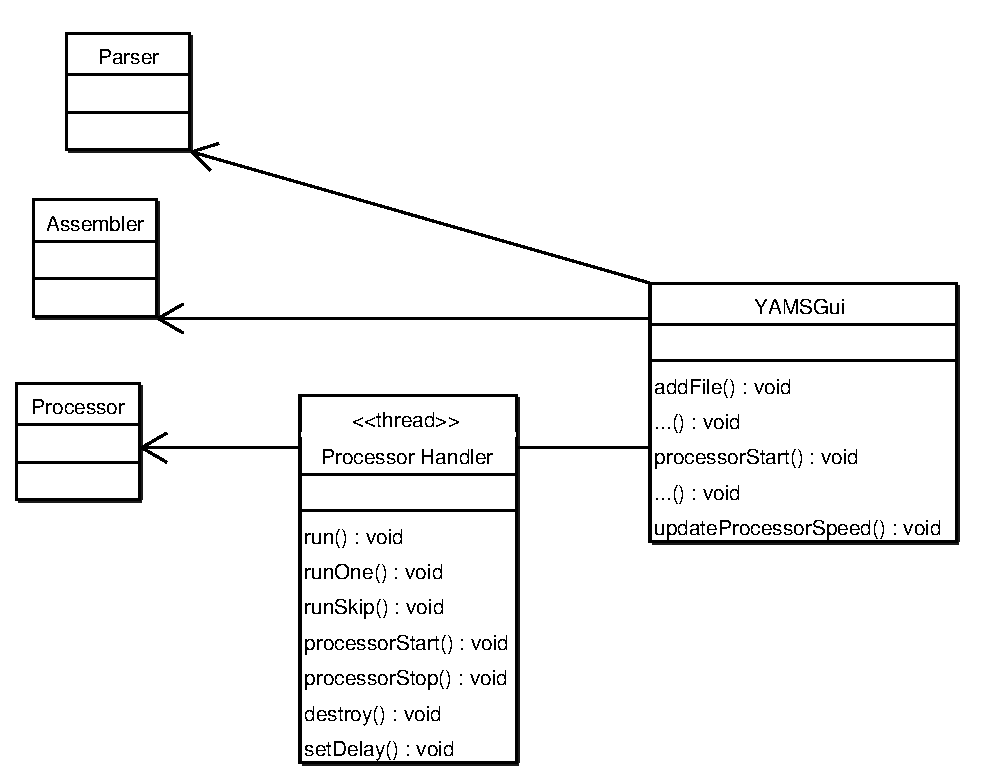
\includegraphics[width=10cm]{ProcessorHandler.eps}
\end{center}
\caption{Processor Handler}
\label{figLineList}
\end{figure}

